\documentclass[10pt,a4paper]{article}
\usepackage[T1]{fontenc}
\usepackage{lmodern,microtype,graphicx,booktabs,tabularx,xcolor}
\usepackage[margin=20mm,top=17mm,bottom=18mm,footskip=9mm]{geometry}
\usepackage[colorlinks=true,urlcolor=teal!60!black]{hyperref}
\usepackage{fancyhdr}
\definecolor{ink}{HTML}{162E38}
\definecolor{accent}{HTML}{076B71}
\definecolor{muted}{HTML}{48616B}
\setlength{\parindent}{0pt}
\setlength{\parskip}{5pt}
\raggedbottom
\pagestyle{fancy}\fancyhf{}
\renewcommand{\headrulewidth}{0pt}
\lfoot{\footnotesize\sffamily\color{muted}Public observations\enspace/\enspace20 November 2026}
\rfoot{\footnotesize\sffamily\color{muted}\thepage}
\newcommand{\kicker}[1]{{\sffamily\small\bfseries\color{accent}#1}\par\vspace{5pt}}
\newcommand{\headline}[1]{{\raggedright\sffamily\bfseries\color{ink}\fontsize{23}{26}\selectfont #1\par}\vspace{3pt}}
\newcommand{\sub}[1]{\par\vspace{3pt}{\sffamily\bfseries\large\color{ink}#1}\par}
\newcommand{\captiontext}[1]{{\small\color{muted}#1}\par}
\begin{document}
\color{ink}
\kicker{SEISMOLOGY \hfill IMPERIAL VALLEY, CALIFORNIA}
\headline{A small earthquake between listed events in the Brawley swarm}
At about \textbf{03:30:02 UTC on 10 May 2026}, ten seismic stations recorded waves that closely resemble those of a cataloged magnitude 1.96 earthquake 13 minutes earlier. The nearest published regional origin is 74 seconds later. The new signal is consistent with a small earthquake near the reference event, of approximate magnitude 1.4.

\begin{center}
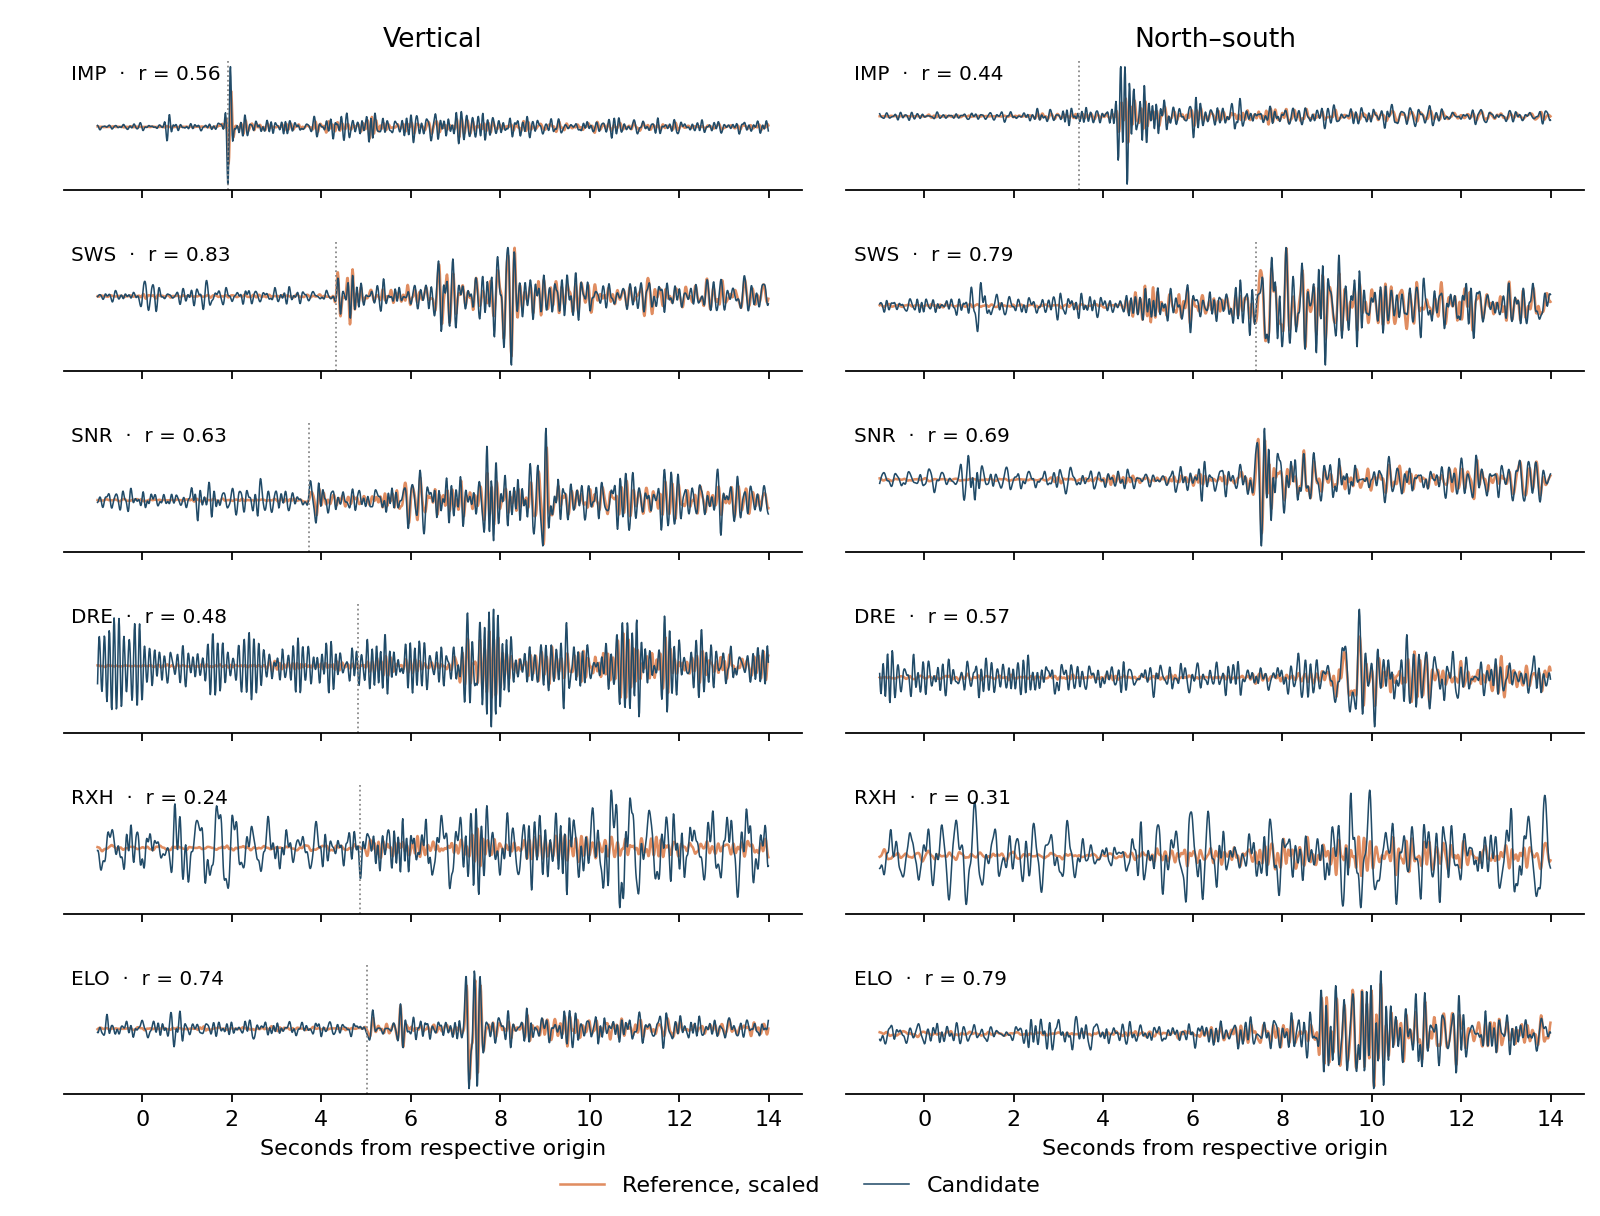
\includegraphics[width=.75\linewidth]{waveforms.png}
\end{center}
\captiontext{Each row shows a different station. Blue is the candidate and orange is the scaled reference. The vertical records were used in discovery and ranking. The horizontal records provide a separate check.}

\sub{Why interpret this as an earthquake?}
A two-hour search with 65 local event templates produced 142 peaks outside the catalog exclusion windows. Three stations detected the candidate and three additional stations ranked it first. The compressional arrivals at those six stations match the reference within 0.02\,s. Two horizontal shear arrivals correlate at 0.96 and 0.90. Shifting the ranking network in time and repeating the ranking produced four maxima at least as large across 7,199 shifts. This describes the local comparison and its search procedure.

Four additional stations across three networks had usable records at the expected arrivals. All three additional horizontal shear-wave correlations exceeded every one of 595 fixed-time control placements per channel. Six station amplitude ratios give relative magnitude estimates of 1.28--1.66. A separate hypocentral fit and calibrated magnitude are still needed.

\sub{What do the public catalogs say?}
The regional network catalog, the dedicated 635-event Brawley relocation catalog, Mexico's RESNOM, USGS ComCat, ISC and EMSC contain no matching local origin. The nearest is at 03:31:16 UTC. Several services share origins. The physical detection and its current catalog status can both be checked against the archived observations. First recognition by any person cannot be established from those records.

\captiontext{Sources: \href{https://doi.org/10.7909/C3WD3xH1}{Southern California Earthquake Data Center}, \href{https://service.scedc.caltech.edu/ftp/catalogs/SCSN_DD/Brawley_hypodd_cat}{Brawley relocation catalog}, \href{https://service.scedc.caltech.edu/fdsnws/event/1/query?eventid=41460424&includearrivals=true}{reference picks CI41460424}, and \href{https://resnom.cicese.mx/sitio/ui/img/Boletines/Reporte_Sec_20260510.pdf}{CICESE swarm bulletin}. The companion files supply waveform windows, selection tables, control trials, catalog extracts and reproducible measurements.}
\end{document}
